%# -*- coding: utf-8-unix -*-
%%==================================================
%% chapter02.tex for SJTU Bachelor Thesis
%%==================================================

%\bibliographystyle{sjtu2}%[此处用于每章都生产参考文献]

\chapter{增强学习算法}
\label{chap:RL}
增强学习属于机器学习算法的一个分支,它研究一个agent如何在交互式环境中连续地做出一系列动作,以获得最大累积奖励的问题。一般而言,增强学习将问题建模成一个马尔可夫决策过程,并有以下组成部分:状态空间$\mathcal{S}$,动作空间$\mathcal{A}$,状态转移概率$\mathcal{P}$和一个回报函数$r:\mathcal{S} \times \mathcal{A} \rightarrow \mathbb{R}$。对于状态-动作空间内的任意轨迹$s_1, a_1, s_2, a_2, ... , s_T, a_T$,状态转移满足马尔可夫性质:$Pr(s_{t+1}|s_1, a_1, ... , s_t, a_t) = Pr(s_{t+1}|s_t, a_t)$。当agent在状态$s$下选择了动作$a$,它会收到环境返回的奖励值$r$(可能为负值)并进入一个新的状态$s'$。在这个过程中,agent选择动作的方式被称为策略。
\section{基于值函数的增强学习}
\subsection{深度模型DQN}
基于值函数的增强学习算法主要有以下几种:Q-Learning,Sarsa和DQN。这里的值函数由$Q$来表示,我们定义$Q(s,a)$为:对状态$s$下选择动作$a$的总回报的估计。在状态空间和动作空间有限时,一定存在某种策略是最优的,即该策略在每个状态下总能选择获得最多奖励(最终累积)的动作,我们将这样的最优策略的$Q$函数记为$Q^*$。如果我们得到了$Q^*$,那么策略的选取将会非常简单:在每个状态$s$下采用贪婪策略,即选择使$Q^*$最大的动作$a$。因此我们的目标就是找到一个对$Q^*$的较好的估计,并采取贪婪策略执行动作。考虑到较后面的动作产生的奖励对最开始的动作的$Q$值影响较小,我们引入折扣因子$\gamma$,那么就有
\begin{equation}
    Q^*(s,a) = r_1 + \gamma r_2 + \gamma^2 r_3 + \gamma^3 r_4 + ...
\label{eq:Q*-1}
\end{equation}
其中,$\gamma$控制了状态$s$下$Q$取决于未来的程度,同时反映了agent预判未来动作带来回报的能力,通常我们设置$\gamma$为一个接近但小于1的数。我们可以将式\ref{eq:Q*-1}写成递归的形式:
\begin{equation}
    Q^*(s,a) = r_1 + \gamma(r_2 + \gamma r_3 + \gamma^2 r_4 + ...) = r_0 + \gamma \max_a Q^*(s,a)
    \label{eq:Q*-2}
\end{equation}
事实上,上式就是一个贝尔曼方程 (Bellman equation)。我们可以将式\ref{eq:Q*-2}改写成值函数的通式:$Q(s,a) = r + \gamma \max_a Q(s,a)$。Watkins和Dayan证明了\cite{watkins1988q}只要状态空间是有限的,且每个状态-动作对都能重复出现,值函数$Q$就可以收敛到$Q^*$。Q-Learning和Sarsa算法通过在环境中的大量摸索,可以将$Q$表(即值函数,一个以状态$s$为列,以动作$a$为行的表)中的值不断更新,直到收敛至$Q^*$。
\begin{figure}[ht]
    \centering
    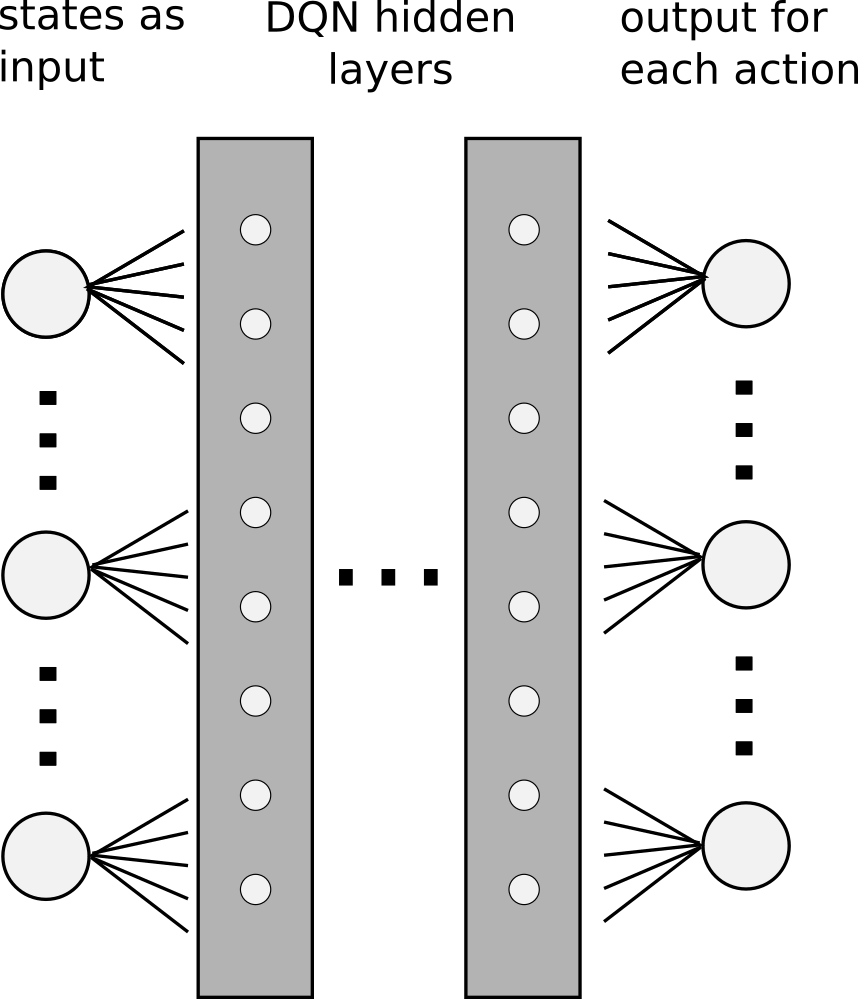
\includegraphics[height=5cm]{figure/dqn.png}
    \caption{Deep Q-Network结构图}
    \label{fig:dqn}
\end{figure}
然而通常情况下,状态空间可能不是有限的,此时$Q$表就是一张无限大的表,我们不可能建立这样一张表并更新其中的值。我们知道,理论上神经网络可以对任意函数进行估计,因此我们考虑用神经网络估计值函数$Q$。该网络的输入是状态$s$,输出是对每个动作$a$的值函数$Q$的估计。如图\ref{fig:dqn}所示,当神经网络有很多层时,这种算法就是Deep Q-Network (DQN)。

\subsection{经验回放}
尽管我们可以用神经网络估计$Q$值,但是此时Watkins和Dayan的结论就不成立了。Volodymyr Mnih等研究者指出:使用神经网络表示值函数$Q$是不稳定的 \cite{hado2012double}。由此他们引入了一些能够使训练稳定的非常有用的机制,其中就包含经验回放 (experience replay)。

在agent的学习过程中,它在某个状态$s$下执行了动作$a$,收到即时奖励$r$并到达下一个状态s'。注意到这种模式是不断重复的:($s, a, r, s'$),若我们的优化过程是即时发生的(产生一个上述四元组就对网络参数更新一次)那么这种学习模式就是online的。由于神经网络不能直接对$Q(s,a)$赋值,我们采用梯度下降算法使$Q(s,a)$向$r + \gamma \max_a Q(s',a)$不断靠近,通过多次重复该过程,agent就获得了越来越多的正确信息,并使它的策略向最优策略收敛。然而这种online的学习也存在着一些问题:($s, a, r, s'$)四元组由于是连续产生的,它们彼此之间的相关性很高,因此可能会导致神经网络的过拟合以致不能有很好的泛化能力;对经验的使用较为低效,这是由于每个四元组只使用了一次。经验回放机制可以较好的解决这个问题:通过对这些状态转移的存储,在学习过程中我们可以从四元组库中随机选取minibatch并计算梯度以更新网络参数(加入经验回放机制的DQN如算法\ref{alg}所示)。

\begin{algorithm}[h]
\begin{algorithmic}
\State Initialize replay memory $\mathcal{D}$ to capacity $N$
\State Initialize action-value function $Q$ with random weights
%\State Require preprocessor $h(s)$ that maps histories to fixed-length representations.
\For{episode $=1,M$} 
\State Initialise sequence $s_1 = \{x_1\}$ and preprocessed sequenced $\phi_1 = \phi(s_1)$
\For {$t=1,T$}
	\State With probability $\epsilon$ select a random action $a_t$
	\State otherwise select $a_t = \max_{a} Q^*(\phi(s_t), a; \theta)$
	\State Execute action $a_t$ in emulator and observe reward $r_t$ and image $x_{t+1}$
	\State Set $s_{t+1} = s_t,a_t,x_{t+1}$ and preprocess $\phi_{t+1} = \phi(s_{t+1})$
	\State Store transition $\left(\phi_t,a_t,r_t,\phi_{t+1}\right)$ in $\mathcal{D}$
	%\For {$k=1$ to $K$}
	\State Sample random minibatch of transitions $\left(\phi_j,a_j,r_j,\phi_{j+1}\right)$ from $\mathcal{D}$
	\State Set
	$y_j =
    \left\{
    \begin{array}{l l}
      r_j  \quad & \text{for terminal } \phi_{j+1}\\
      r_j + \gamma \max_{a'} Q(\phi_{j+1}, a'; \theta) \quad & \text{for non-terminal } \phi_{j+1}
    \end{array} \right.$
	\State Perform a gradient descent step on $\left(y_j - Q(\phi_j, a_j; \theta) \right)^2$
	%\EndFor
\EndFor
\EndFor
\end{algorithmic}
\caption{Deep Q-learning with Experience Replay \cite{hado2011double}}
\label{alg}
\end{algorithm}

\subsection{Double DQN}
我们知道,DQN由于是Q-learning的扩展而包含了$\max_a Q^*(s,a)$,而在训练过程中的$Q$是神经网络在当前状态下对于值函数的预测,并不是真实的最优值,那么对$Q$取max就有可能包含了$Q$值的最大误差,直接用它对此时的神经网络更新参数就会带来overestimate的问题。Hado van Hasselt等人在2016年通过引入Double Q-learning \cite{hado2010double} 提出了Double DQN \cite{hado2016deep}的概念,很好地解决了这个问题。他们将原来DQN中使用同一个神经网络选择、评价动作的过程分离,在t时刻下分别用参数为$\theta_t$的最新的online神经网络估计值函数$Q$、用参数为$\theta'_t$的神经网络评价该策略的值(即计算loss以实现$\theta_t$网络的梯度反向传播),事实上我们每隔一段时间用$\theta_t$为$\theta'_t$更新参数。具体而言,$\theta_t$神经网络的更新目标$Y^{\text{DoubleQ}}_t$是:
\begin{equation}
Y^{\text{DoubleQ}}_t \!\equiv r_{t} + \gamma Q(s_{t+1}, \argmax_a Q(s_{t+1}, a; \theta_t); \theta'_t )
\label{doubledqn}
\end{equation}
其中$r_{t}$是即时奖励,$\argmax_a Q$是由$\theta_t$网络对下一步动作的选择,这意味着和Q-learning相同,此处依然根据当前的网络参数估计、使用贪婪策略选择动作。
\section{基于策略的增强学习}
基于值函数的增强学习算法得到的是给定某状态下每种动作的$Q$值,agent选择$Q$值最大的动作(贪婪策略下)。与基于值函数的算法不同,基于策略的增强学习不输出某状态下的动作的值,而是直接输出具体的某个动作,即直接对策略进行建模。基于策略的增强学习算法按输出分为两类:Stochastic方法输出动作空间$\mathcal{A}$上的概率分布,Deterministic方法直接输出动作$a$本身。

\subsection{Stochastic策略梯度方法}
\label{sec:stochas_PG}
在此种方法中,agent的动作由随机(stochastic)策略$\pi (s)$决定。随机策略的意思是它不输出一个单独的动作,而是输出各种动作的概率分布,所有动作的概率之和为1。我们采用$\pi (a|s)$表示状态$s$下选择动作$a$的概率。简单而言,策略$\pi$并不最大化任何值,只是对于某个状态s给出所有可能动作的概率。策略$\pi$的价值函数定义为折扣回报的期望:
\begin{equation}
V(s) = E_{\pi (s)}[r + \gamma V(s’)]
\end{equation}
这里我们对状态s下的所有可能动作的$r + \gamma V(s’)$取平均(而没有取最大值)。另外我们定义一个优势函数$A(s, a)$:$A(s,a) = Q(s,a) - V(s) $。显然,这个函数的意义是:在状态s下采取动作a带来的回报比动作空间的回报均值多出了多少。最后我们用$\rho$来表示状态的分布,即在某种状态的概率,那么$\rho^{s_0}$就是环境初始状态的概率分布,$\rho^\pi$则是在采取某策略$\pi$下的状态分布。
%\begin{comment}
%\begin{algorithm}[h]
%  \caption{Reinforce Algorithm \cite{reinforce}} 
%  \label{algo:reinforce}
%  \begin{algorithmic}
%    \State Initialize $\theta$ arbitrarily.
%    \For{$episode = {s_1, a_1, r_1, ..., s_T, a_t} \sim \pi_\theta$}
%      \For{t = 1 to T-1}
%        \state $\theta \leftarrow \theta + \alpha \Delta_\theta log \pi_\theta(s_t, a_t)v_t$
%      \EndFor
%    \EndFor
%  \end{algorithmic}
%\end{algorithm}
%\end{comment}
与Deep Q-Network的想法类似,我们同样可以用神经网络(参数为$\theta$)估计策略(即一个以状态$s$为输入、动作概率分布$\pi_\theta$为输出的函数)。agent可以根据输出的动作概率选择下一步的动作。为了优化策略,我们需要定义衡量策略好坏的函数$J(\pi)$:
\begin{equation}
J(\pi) = E_{\rho^{s_0}}[V(s_0)]
\end{equation}
$J(\pi)$可以告诉我们对于所有可能的初始状态一个策略能够获得的折扣回报的平均值。根据策略梯度定理\cite{sutton1999policy},我们知道$J(\pi)$的梯度可以轻易由下面的式子计算得到:
\begin{equation}
\begin{split}
\nabla_\theta J(\pi_\theta) = \int_\mathcal{S}\rho^{\pi_\theta}(s)\int_\mathcal{A}\nabla_\theta \pi_\theta(a\vert s)Q^{\pi_\theta}(s,a) \texttt{d}a\texttt{d}s \\  = \mathbb{E}_{s\sim \rho^{\pi_\theta},a\in \pi_\theta}[\nabla_\theta log \pi_\theta(a\vert s)A(s,a)]
\end{split}
\label{stotheorem}
\end{equation}
式\ref{stotheorem}提供了神经网络参数更新的方向:$\nabla_\theta log \pi_\theta(a\vert s)$是状态$s$下选择动作$a$的概率增加的方向,$A(s,a)$是选择该动作的优势,两项结合起来就是得到比平均回报的多的动作的概率增加,得到比平均回报少的动作的概率减小。尽管我们不能对每一个状态和动作计算策略梯度,我们提前产生大量的样本,这些样本服从与期望值相接近的概率分布(可证明agent在环境中运行时所遇到的状态和执行的动作是服从$\rho^\pi$和$\pi(s)$的无偏差样本)。当我们收集了agent的足够多的四元组$(s,a,r,s’)$时,通过计算式\ref{stotheorem},我们就可以使用梯度下降算法更新神经网络参数,提升策略的表现。
\subsection{Deterministic策略梯度方法}
Deterministic策略梯度方法\cite{silver2014deter}是2014年最先由David Silver等人提出的,他们考虑了一种决定性策略$a = \mu_\theta(s)$,即以$\theta$为参数的神经网络以状态$s$为输入,直接输出动作$a$。我们首先定义从$t$时刻开始的总折扣回报(total discounted reward)$r^\gamma_t$:
\begin{equation}
r^\gamma_t = \sum^\infty_{k=t}\gamma^{k-t} r(s_k,a_k), 0<\gamma<1
\end{equation}
与Stochastic策略梯度方法相似,我们定义一个衡量策略表现的函数$J(\mu_\theta) = \mathbb{E}[r^\gamma_1 \vert \mu_\theta]$(其意义就是在策略$\mu_\theta$下,从初始时刻$t=1$开始的总折扣回报的期望)和折扣状态分布$\rho^{\mu_\theta}(s)$。这样我们就有:
\begin{equation}
\begin{split}
J(\mu_\theta) = \int_\mathcal{S}\rho^{\mu_\theta}(s) r(s, \mu_\theta(s))\texttt{d}s = \mathbb{E}_{s\sim \rho^{\mu_\theta}}[r(s, \mu_\theta(s)]
\end{split}
\label{detobj}
\end{equation}
Silver等人证明了决定性的策略梯度定理,打破了使决定性策略梯度算法变为可能:
\begin{equation}
\begin{split}
\nabla_\theta J(\mu_\theta) = \int_\mathcal{S}\rho^{\mu_\theta}(s)\nabla_\theta \mu_\theta(s) \nabla_a Q^{\mu_\theta}(s,a) \vert_{a = \mu_\theta(s)} \texttt{d}s \\  = \mathbb{E}_{s\sim \rho^{\mu_\theta}}[\nabla_\theta \mu_\theta(s) \nabla_a Q^\mu(s,a) \vert_{a = \mu_\theta(s)}]
\end{split}
\label{dettheorem}
\end{equation}
通过使用式\ref{dettheorem},我们就能够像随机策略梯度算法一样更新神经网络参数,利用agent在环境中得到的大量$(s,a,r,s’)$样本优化策略。
\section{Actor-Critic方法}
回顾基于值函数和基于策略的增强学习算法,我们发现它们都是利用神经网络来估计某个函数。那么我们不妨将二者结合起来,使用相同的神经网络,既估计策略本身又估计策略的价值函数。这样做有很多好处:我们同时优化两个目标函数可以使学习过程更快更有效;一同优化两个目标可以相互起到规范化的作用,带来训练过程中更大的稳定性。
\begin{figure}
    \centering
    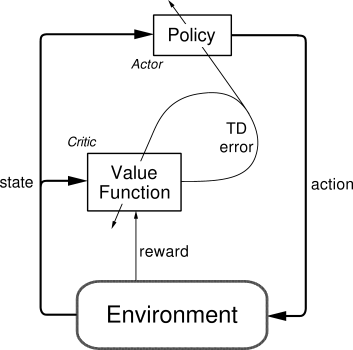
\includegraphics[height=6cm]{figure/actor-critic.png}
    \caption{Actor-Critic结构图}
    \label{fig:actor-critic}
\end{figure}
\subsection{DPG算法}
\label{sec:DPG}
David Silver等人提出的DPG (Deterministic Policy Gradient)\cite{silver2014deter}算法都属于决定性的actor-critic算法。DPG能够很好地解决连续动作空间上的问题,主要分为on-policy和off-policy两种。On-policy算法中的critic负责估计动作的价值函数(这里使用一个可微的动作价值函数$Q^\omega(s,a)$替换真实的动作价值函数$Q^\mu(s,a)$,并使用Sarsa算法对其参数进行更新),actor负责通过策略梯度算法调整决定性策略$\mu_\theta(s)$。Off-policy算法与On-policy算法的不同之处在于critic的参数更新算法使用了Q-learning。Silver等人通过计算得到了衡量策略表现的函数$J$的梯度\cite{silver2014deter}(如式\ref{dpg_act}所示),由此DPG算法的actor就可以对折扣回报的期望应用链式法则以更新actor参数。
\begin{equation}
\begin{split}
  \nabla_{\theta^\mu} J &\approx
  \mathbb{E}_{s \sim \rho^{\mu_\theta}}\left[\nabla_{\theta^{\mu}}
    Q(s, a | \theta^Q)|_{s = s_t, a = \mu(s_t | \theta^{\mu})}
                   \right] \\
                 & =
    \mathbb{E}_{s \sim \rho^{\mu_\theta}}\left[\nabla_{a} Q(s, a | \theta^{Q})|_{s = s_t, a = \mu(s_t)}
    \nabla_{\theta_\mu} \mu(s | \theta^{\mu})|_{s = s_t} \right]
\end{split}
\label{dpg_act}
\end{equation}

\subsection{DDPG算法}
DDPG (Deep Deterministic Policy Gradient)\cite{timothy2016cont}算法是使用深度神经网络对DPG (Deterministic Policy Gradient)\cite{silver2014deter}中Off-policy算法的扩展,它与DPG一样都属于actor-critic算法。DDPG一共包含四个相互关联的深度神经网络,其中两个是对DPG中的actor $\theta^\mu$和critic $\theta^Q$分别进行估计的神经网络,另外两个来自如式\ref{doubledqn}中选择与评价分离机制(Double DQN的思想)的两个目标网络$\theta^{\mu'}$和$\theta^{Q'}$。训练过程中,$\theta^\mu$和$\theta^Q$都采用如算法\ref{alg}中的经验回放机制,对记忆库中的$(s_i,a_i,r_i,s_{i+1})$四元组采样出大小为$N$的minibatch,以避免时间上邻近的样本之间的相关性带来的网络过拟合情况。critic网络的损失函数$L$的计算过程如算法\ref{dpgalgo}所示,首先用$\theta^{\mu'}$和$\theta^{Q'}$计算目标$y$,再用当前的$\theta^{Q}$估计值函数$Q$,再对二者作差。actor网络参数的更新与DPG算法的式\ref{dpg_act}相同。

目标网络$\theta^{\mu'}$和$\theta^{Q'}$的训练采用一种平滑的更新机制,通过设置$\tau$,它们的参数缓慢地跟着$\theta^{\mu}$和$\theta^{Q}$更新:$\theta' \leftarrow \tau\theta + (1 - \tau) \theta'$, $\tau \ll 1$。这意味着目标网络参数的改动是被限制的,这能够提升学习过程的稳定性\cite{timothy2016cont}。对于agent观察到的环境是用低维特征向量表示的场景,不同的特征向量可能具有不同的物理单位,因而使用一个网络对不同尺度的输入进行建模是困难的。Timothy P. Lillicrap等人利用批标准化技术 (batch normalization\cite{ioffe2015batch})解决了这一问题。在低维的情形下,他们对状态输入、$\theta_\mu$网络的所有层、$\theta_Q$网络的所有层应用了批标准化,抑制了差异值偏差 (covariate shift)在训练过程中的扩大,进而可以缓解训练中的梯度消失 (gradient vanishing)问题。另外,连续的动作空间中很容易出现agent对环境探索不足的问题,但由于DDPG采用Off-policy机制,agent对于环境的探索与学习算法是分离的,因而可以对策略$\mu$引入噪声,每个时刻的噪声从一个噪声随机过程$\mathcal{N}$中采样得到:
\begin{equation}
  \mu'(s_t) = \mu(s_t | \theta^\mu_t) + \mathcal{N}
\end{equation}
其中$\mathcal{N}$是一种适应于agent所处环境的Ornstein-Uhlenbeck过程\cite{uhlenbeck1930on}。该过程具有时间互相关性,适合于增强学习的场景。



\begin{algorithm}[h]
  \caption{Deep Deterministic Policy Gradient \cite{timothy2016cont} \label{algo:ddpg}}
  \label{dpgalgo}
  \begin{algorithmic}
    \State Randomly initialize critic network $Q(s, a | \theta^Q)$ and actor
    $\mu(s | \theta^{\mu})$ with weights $\theta^{Q}$ and $\theta^{\mu}$.
    \State Initialize target network $Q'$ and $\mu'$ with weights $\theta^{Q'}
    \leftarrow \theta^{Q}$, $\theta^{\mu'} \leftarrow \theta^{\mu}$
    \State Initialize replay buffer $R$
    \For{episode = 1, M}
      \State Initialize a random process $\mathcal{N}$ for action
      exploration
      \State Receive initial observation state $s_1$
      \For{t = 1, T}
        \State Select action $a_t = \mu(s_t | \theta^{\mu}) + \mathcal{N}_t$
        according to the current policy and exploration noise
        \State Execute action $a_t$ and observe
        reward $r_t$ and observe new state $s_{t+1}$
        \State Store transition $(s_t, a_t,
                r_t, s_{t+1})$ in $R$
        \State Sample a random minibatch of $N$ transitions
               $(s_i, a_i,
        r_i, s_{i + 1})$ from $R$
        \State Set $ y_i = r_i + \gamma Q'(s_{i + 1},
        \mu'(s_{i+1} | \theta^{\mu'}) | \theta^{Q'}) $
            %\begin{cases}
            %r_t + \gamma Q'(\mathbf{s}_{j + 1}, \mu'(\mathbf{s}_{j+1})) &
            %                      \text {for non terminal } \\
            %                      r_t & \text{ for terminal } \\
            %\end{cases} $
        \State Update critic by minimizing the loss:
               $L = \frac{1}{N} \sum_i (y_i -
               Q(s_i, a_i | \theta^Q))^2$
        \State Update the actor policy using the sampled policy gradient:
        \begin{equation*}
            \nabla_{\theta^{\mu}} J \approx
            \frac{1}{N} \sum_i
               \nabla_{a} Q(s, a | \theta^Q)|_{s = s_i, a = \mu(s_i)}
               \nabla_{\theta^\mu} \mu(s | \theta^\mu)|_{s_i}
         \end{equation*}
        \State Update the target networks:
          \begin{equation*}
            \theta^{Q'} \leftarrow \tau \theta^{Q} + (1 - \tau) \theta^{Q'}
          \end{equation*}
          \begin{equation*}
            \theta^{\mu'} \leftarrow \tau \theta^{\mu} +
                (1 - \tau) \theta^{\mu'}
          \end{equation*}
        \EndFor
    \EndFor
  \end{algorithmic}
\end{algorithm}
